% ---------------------------------------------------
%
% Trabajo de Fin de Grado. 
% Author: Adriano dos Santos Moreira
% Chapter: Full SYCL Implementation
% File: Cap5_Full_SYCL_Implementation.tex
%
% ----------------------------------------------------
%

\chapter{An Industry Case Study: Image Processing with SYCL} \label{chap:CaseStudy} 

In this chapter we will take a deep look into the development of a SYCL application.
For this purpose, we have contacted Wooptix\footnote{\url{https://wooptix.com}}, a Canary Islands based company with expertise in image processing.
To illustrate their needs, Wooptix suggested the implementation of the erosion operation on FITS format images and they provided us with one of the images they use for real purposes.

The erosion is one of the fundamental operations in morphological image processing \cite{Gonzalez:2008:Digital}.
This branch of knowledge studies the structure and components of an image with the objective of creating useful descriptions of its shape, while also providing tools for signal processing.

On the other hand, the FITS (Flexible Image Transport System) file format is the standard astronomical data format supported by NASA and the IAU (International Astronomical Union).
This standard supports multi-dimensional images, although we will only focus on two-dimensional FITS files.

The application presented in this chapter was developed using C++.
To open and process images in FITS format, we will use CFITSIO\footnote{\href{https://heasarc.gsfc.nasa.gov/fitsio/}{{FITSIO Home Page} \url{https://heasarc.gsfc.nasa.gov/fitsio/}}}, a library of C and Fortran subroutines for reading and writing FITS files.

\section{The erosion operation}

The erosion operation is used to shrink or erode the boundaries of objects within an image applying a structuring element.

\vspace{5mm}
\textsl{\textbf{{Structuring Element}}}
\vspace{2mm}

A structuring element (SE) is a mask which determines how the operation is applied to the image.
This object is usually represented by a matrix, where non-zero values describe the mask and a center origin to apply the mask from.
We can classify them in two types:
\begin{itemize}
    \item \textbf{Flat SE}: Composed of 0s and 1s only, simply establishes which pixels are relevant and which are not.
    \item \textbf{Non-flat SE}: Contains grayscale values that describe how meaningful the pixels are.
\end{itemize}

For this application, we will work with two-dimensional grayscale images using flat structuring elements.

The erosion operation consists of sliding a SE over an entire image, applying the SE to each pixel.
This procedure takes the lowest value in the vicinity established by the SE (with a value of 1) and assigns it to the evaluated pixel, creating an output image whose bright regions are shrunk and dark regions are enlarged.

\begin{figure}[H]
    \centering
    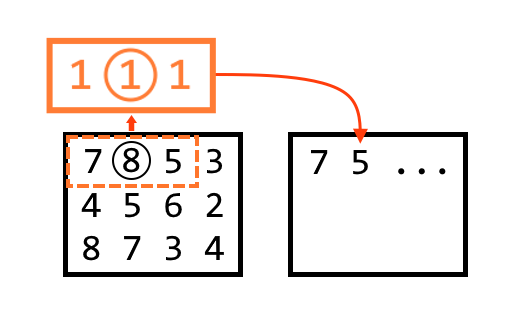
\includegraphics[width=0.5\linewidth]{images/erosion_graph.png}
    \caption{Simplified erosion operation.}
    \label{fig:erosion-graph}
\end{figure}

In Figure \ref{fig:erosion-graph} we can see a graphical example of this transformation.
In this illustration, the second element of the input image is evaluated.
According to the SE, the neighborhood of the element is 7, 8 and 5, from which we can conclude that the lowest value is 5, resulting in the value of erosion at the second pixel.

Note that certain border regions of the image make the SE go out of bounds.
In order to process image borders correctly, we add padding around the image with a very high value, ensuring that the algorithm only considers pixels within the original image.
\pagebreak
\section{Supporting Code}

In order to implement the erosion operation, we need to create an environment to work on images in FITS format, as well as to represent the structuring element and make everything work together.

The supporting code is based on three main classes:
\begin{itemize}
    \item \texttt{FitsImage}: Encapsulates the functionality of the CFITSIO library.
    \item \texttt{StructuringElement}: Represents a SE and provides access to every detail of it.
    \item \texttt{Morphology}: Base class for the morphology operations, this makes the project easily expandable.
\end{itemize}

One important aspect to note is that the FITS format supports many pixel sizes, so the number of bytes a pixel occupies may vary from file to file.
This is important to have into account because we need to maintain format consistency when reading, operating and writing the image we work with.

Depending on the pixel size, the application will decide on a data type in runtime, which can be one of the following: \texttt{unsigned char}, \texttt{short}, \texttt{long}, \texttt{long long}, \texttt{float} or \texttt{double}.

Because we are using C++, we need to use polymorphism in combination with the factory method pattern\footnote{\href{https://refactoring.guru/design-patterns/factory-method}{{Factory method} \url{https://refactoring.guru/design-patterns/factory-method}}} to achieve dynamic type behaviour in our program.

\begin{figure}[H]
    \centering
    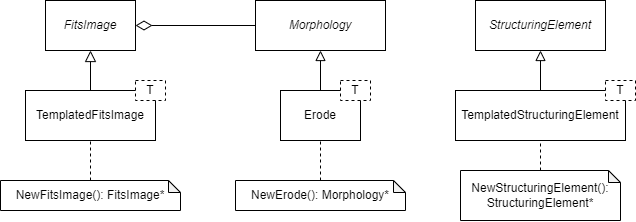
\includegraphics[width=0.85\linewidth]{images/morph_uml.png}
    \caption{Conceptual UML class diagram for the erosion application.}
    \label{fig:uml-morph-graph}
\end{figure}

This dynamic typing was made possible thanks to the implementation of the abstract base classes described in Figure \ref{fig:uml-morph-graph}.
Each of these classes derive in a class template that can be used to dynamically create instances by using a non-member function, also indicated in the diagram with a note for every concrete class.

\section{Erosion Solution Development}

We present two implementations for the erosion operations, this section is dedicated to explain in detail how the operation is performed in both serial and SYCL approaches.

It would be beneficial to keep a few notes in mind when reading the implementations:
\begin{itemize}
    \item Both \texttt{FitsImage} and \texttt{StructuringElement} data are stored in generic type one-dimensional arrays.
    \item Data arrays are stored in row-major order, starting from the bottom left.
    \item The code shown operates directly on the image representation, modifying the \texttt{FitsImage} content.
\end{itemize}

\subsection{Serial Implementation}

The serial implementation of the erosion operation presented here is quite straightforward.
This approach provides a baseline against which the performance of the parallel version can be measured, while also serving as a reference to see whether its parallel version is worth the effort.

In addition, writing a naive implementation can provide insight into the complexity and potential bottlenecks of the algorithm, and help understand how the algorithm scales with increasing data or computational load.

The algorithm can be divided in two main zones.
The first is the preparation for the erosion and the second is the erosion itself.
\pagebreak

\lstinputlisting[language=C++,style=cppstyle,caption={Serial erosion function. \href{{https://github.com/AdrianoMoreira08/TFG-SYCL/blob/main/image-processing/morphology-gray/include/erode.h}}{\textit{See on Github}}.},label={listing:serial-morph-full}]{listings/serial_morph_full.cc}

The first action of the preparation code is to cast both the FITS image and the structuring element pointers into their corresponding concrete class, which have the accessors to the template dependant arrays of data.
This happens in lines 2-5.
Then, lines 6 and 9 retrieve both image and SE data pointers.

We cannot read and write over the same image data, since it would modify the neighbourhood of pixels we will operate on later.
To avoid this situation, we create a copy of the image data in line 8.

To conclude the set-up, we calculate the location of the first pixel of the image in line 10.

The erosion operation itself starts from line 11, where the main loops (lines 11 and 13), traverse the whole image.
After every row, we calculate the first index of said row for the image data array in line 12, and for every column, we obtain the pixel index in line 14 for the pixel we will evaluate.
Another relevant index is the location of the first pixel that corresponds to the SE evaluation, calculated in lines 15-17.

The region of code that covers lines 18-30 determines the output pixel value of the current pixel, which calculates the minimum pixel value in the neighbourhood set by the SE.

Starting in line 18, we set a very high minimum value for the output pixel.
Then, the loops in lines 19 and 22 traverse the whole structuring element.
For every row, we calculate the first index of said row for the image data array as well as for the SE, accomplished in lines 20-21.

In the innermost loop, we compute the neighbour pixel index to be evaluated in line 23 and check if the structuring element considers that pixel and whether its value is the new minimum.
If it passes the checks, the new minimum is assigned in line 26.
After the calculation of the minimum, it is set as the new pixel value in line 30.
As a last action, we delete the copy of the image in line 33.

\subsection{SYCL Implementation}

The parallel implementation using SYCL is based on the naive algorithm presented in the serial implementation.
Nevertheless, a parallel approach to this algorithm is clear to give significant benefits if we take into account the embarrassingly parallel nature of it.
To be more specific, the fact that each pixel of the image is processed independently of each other, makes it an ideal candidate for parallel execution.
Moreover, if we implement memory tiling to this process, the the efficiency can be further enhanced.

Memory tiling involves dividing the image into smaller blocks that fit into the fast, local memory dedicated to every work-group.
By doing so, we can significantly reduce the latency associated with accessing global memory.
Each tile can be loaded into the local memory, processed independently, and then the results can be written back to global memory.
This approach minimizes memory access delays and improves data locality, ensuring that each work-item spends more time computing and less time waiting for data.

For this implementation we will use the buffer/accessor model, covered in Section \ref{sec:buffer-accessor} of Chapter \ref{chap:SYCL}.
\pagebreak

\lstinputlisting[language=C++,style=cppstyle,caption={Set-up for SYCL parallel execution. \href{{https://github.com/AdrianoMoreira08/TFG-SYCL/blob/main/image-processing/morphology-gray/include/erode_sycl.h}}{\textit{See on Github}}.},label={listing:sycl-morph-setup}]{listings/sycl_morph_setup.cc}

In Listing \ref{listing:sycl-morph-setup} we have the preparation code for the kernel execution.
Firstly, we create a queue and select a GPU device in line 1.
Then we retrieve both image and SE pointers and their data (lines 2-7), the same way we did for the serial version.

Lines 9-13 set padding related ranges and offsets.
Line 15 starts the buffer scope, outside of which the buffers are destroyed.

Following, we have two sets of ranges.

In the first one, line 17 specifies the size of the work-groups of the NDRange, which is defined to be the same size as the SE.
Then we define how many work-groups we need by dividing the image dimensions by the local range and taking the ceiling of the result.
This is calculated in lines 18-21.
After this, we can calculate the global range and set the NDRange in lines 22-24.

The second set of ranges calculates buffer sizes.
Both input and output image buffer ranges are the same size (lines 26-29) and is set to the size of the original padded image.
The SE range, in line 30 has the same dimensions as the SE itself.
On the other hand, in line 31, the tile range is set to be the local range plus twice the padding, ensuring that the structuring element does not to surpass the tile range.

The next 33-37 lines simply create the buffers using the previously defined ranges and data pointers.
Note that line 34 indicates that the image buffer has nowhere to write back when the buffer is destroyed, this is specified to ensure that there is no time lost writing unnecessary data back.
On the other hand, line 36 gives the output buffer a pointer to write back to, which is the pointer to the original data array, successfully overwriting the data.
\pagebreak
\lstinputlisting[language=C++,style=cppstyle,firstnumber=38,caption={Erosion operation kernel using SYCL. \href{{https://github.com/AdrianoMoreira08/TFG-SYCL/blob/main/image-processing/morphology-gray/include/erode_sycl.h}}{\textit{See on Github}}.},label={listing:sycl-morph-operation}]{listings/sycl_morph_operation.cc}

The erosion operation occurs in Listing \ref{listing:sycl-morph-operation}, where we submit the command group to the queue (line 39).
Just before the kernel starts, we define a series of accessors in lines 40-42, which correspond to the image (read-only), output (write-only) and SE (read-only).
A fourth accessor is present in line 43, which grants access to the local memory to perform the memory tiling with.

Line 45 starts the definition of the kernel.
First, we set various indexes related to the current work-item (lines 46-49):
\begin{itemize}
    \item \textbf{Global ID}: Unique global identifier.
    It matches with the output pixel index since the \texttt{parallel\_for} range coincides with the image range.
    \item \textbf{Group ID}: Identifies the work-group.
    Useful to calculate where the work-group tile begins within the image.
    \item \textbf{Local ID}: Index of the work-item within the work-group.
    Determines which pixels the work-item has to copy to the tile and the offset to read within the tile.
    \item \textbf{Global group offset}: First index of the tile within the image.
\end{itemize}

In order to write the whole tile, each work-item of the work-group contributes to copy from the image to the tile without repeating.
This is done in lines 52-56, where each work-item starts at a unique position determined by the local ID and iterates in increments of the size of the local range.
This approach ensures that no work item repeats the copy operation on the same pixel.

To guarantee that every work-item has access to the same exact full information of the tile, line 57 sets a group barrier which makes all work-items in the work-group wait until each one has reached this point in the code.
Right after, we calculate the starting point where the SE will be applied within the image.
Line 58 determines this starting point, obtaining the index of the first element to be read, which will serve as an offset in the next calculations.

The computation for the new pixel value starts by setting a very high number as the new minimum in line 61.
Following, we iterate over the SE using loops 62 and 63.
In the innermost loop, we start by identifying which pixel of the image to analyze in line 64.
Then, if the current position of the SE indicates that such pixel may be considered, we evaluate whether the pixel value is the new minimum.
This process happens in lines 65-68.
The new minimum value is written in the output buffer in line 72.

Finally, we wait in line 75 for this task to finish.
\pagebreak

\section{Results}

In this section, we will present the application of the erosion operation on various images.
We will also display the global compute time of each program as well as the isolated time for the operation only.
The code presented in the previous section was run on \textit{Verode}, the same platform described in Chapter \ref{chap:Benchmark_Comparisons}.

The first image we will process was created using the the Faint Object Camera (FOC) from the Hubble Space Telescope in July 1996, with the size of 1024 by 1024 pixels.
This picture is part of a sample collection\footnote{\href{https://fits.gsfc.nasa.gov/fits\_samples.html}{{Sample FITS Files} \url{https://fits.gsfc.nasa.gov/fits\_samples.html}}} listed by NASA.
In Figure \ref{fig:og-foc} we can see this image.

\begin{figure}[H]
    \centering
    \includegraphics[width=0.5\linewidth]{images/og-foc.png}
    \caption{Original FOC sample image.}
    \label{fig:og-foc}
\end{figure}

For this first experimentation, we will use the structuring element shown in Listing \ref{listing:cross-se}. 
It defines a simple cross shape whose chosen center is (1, 1), the second element of the second row.

\begin{tabular}{c}
\lstinputlisting[language=C++,style=cppstyle,caption={Cross-shaped structuring element.},label={listing:cross-se}]{listings/cross.txt}
\end{tabular}

Figure \ref{fig:result-foc} illustrates a magnified comparison of the original (left) and eroded (right) images.
Given that both serial and SYCL implementations yield the same final image, there is no need to display or differentiate the resulting images.

\begin{figure}[H]
    \centering
    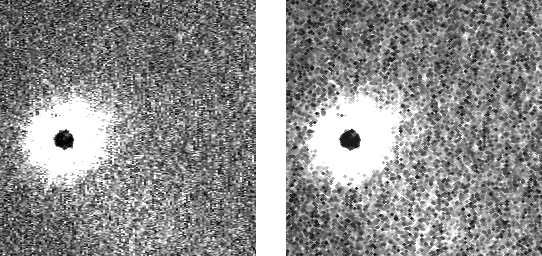
\includegraphics[width=0.7\linewidth]{images/FOC-result.png}
    \caption{Zoomed in FOC image. Original (left) and eroded (right).}
    \label{fig:result-foc}
\end{figure}

Executing both serial and parallel versions 10 times and averaging the times, we find the following results:

\begin{itemize}
    \item The overall program execution time is 1.10 seconds for serial and 1.30 seconds for SYCL.
    \item The operation execution time is 0.04 seconds for serial and 0.17 seconds for SYCL.
\end{itemize}

For this specific test, both overall and operation times are lower for the serial version.
This is expected since smaller images may suffer from the overhead introduced by the parallel SYCL version, while larger images would greatly benefit from the parallel implementation.

To prove that the SYCL implementation can actually outperform the serial version, we worked with a large sample image provided by Wooptix.
The image size is is 6388 by 6388 pixels and you can see it in \ref{fig:og-wooptix}.

\begin{figure}[H]
    \centering
    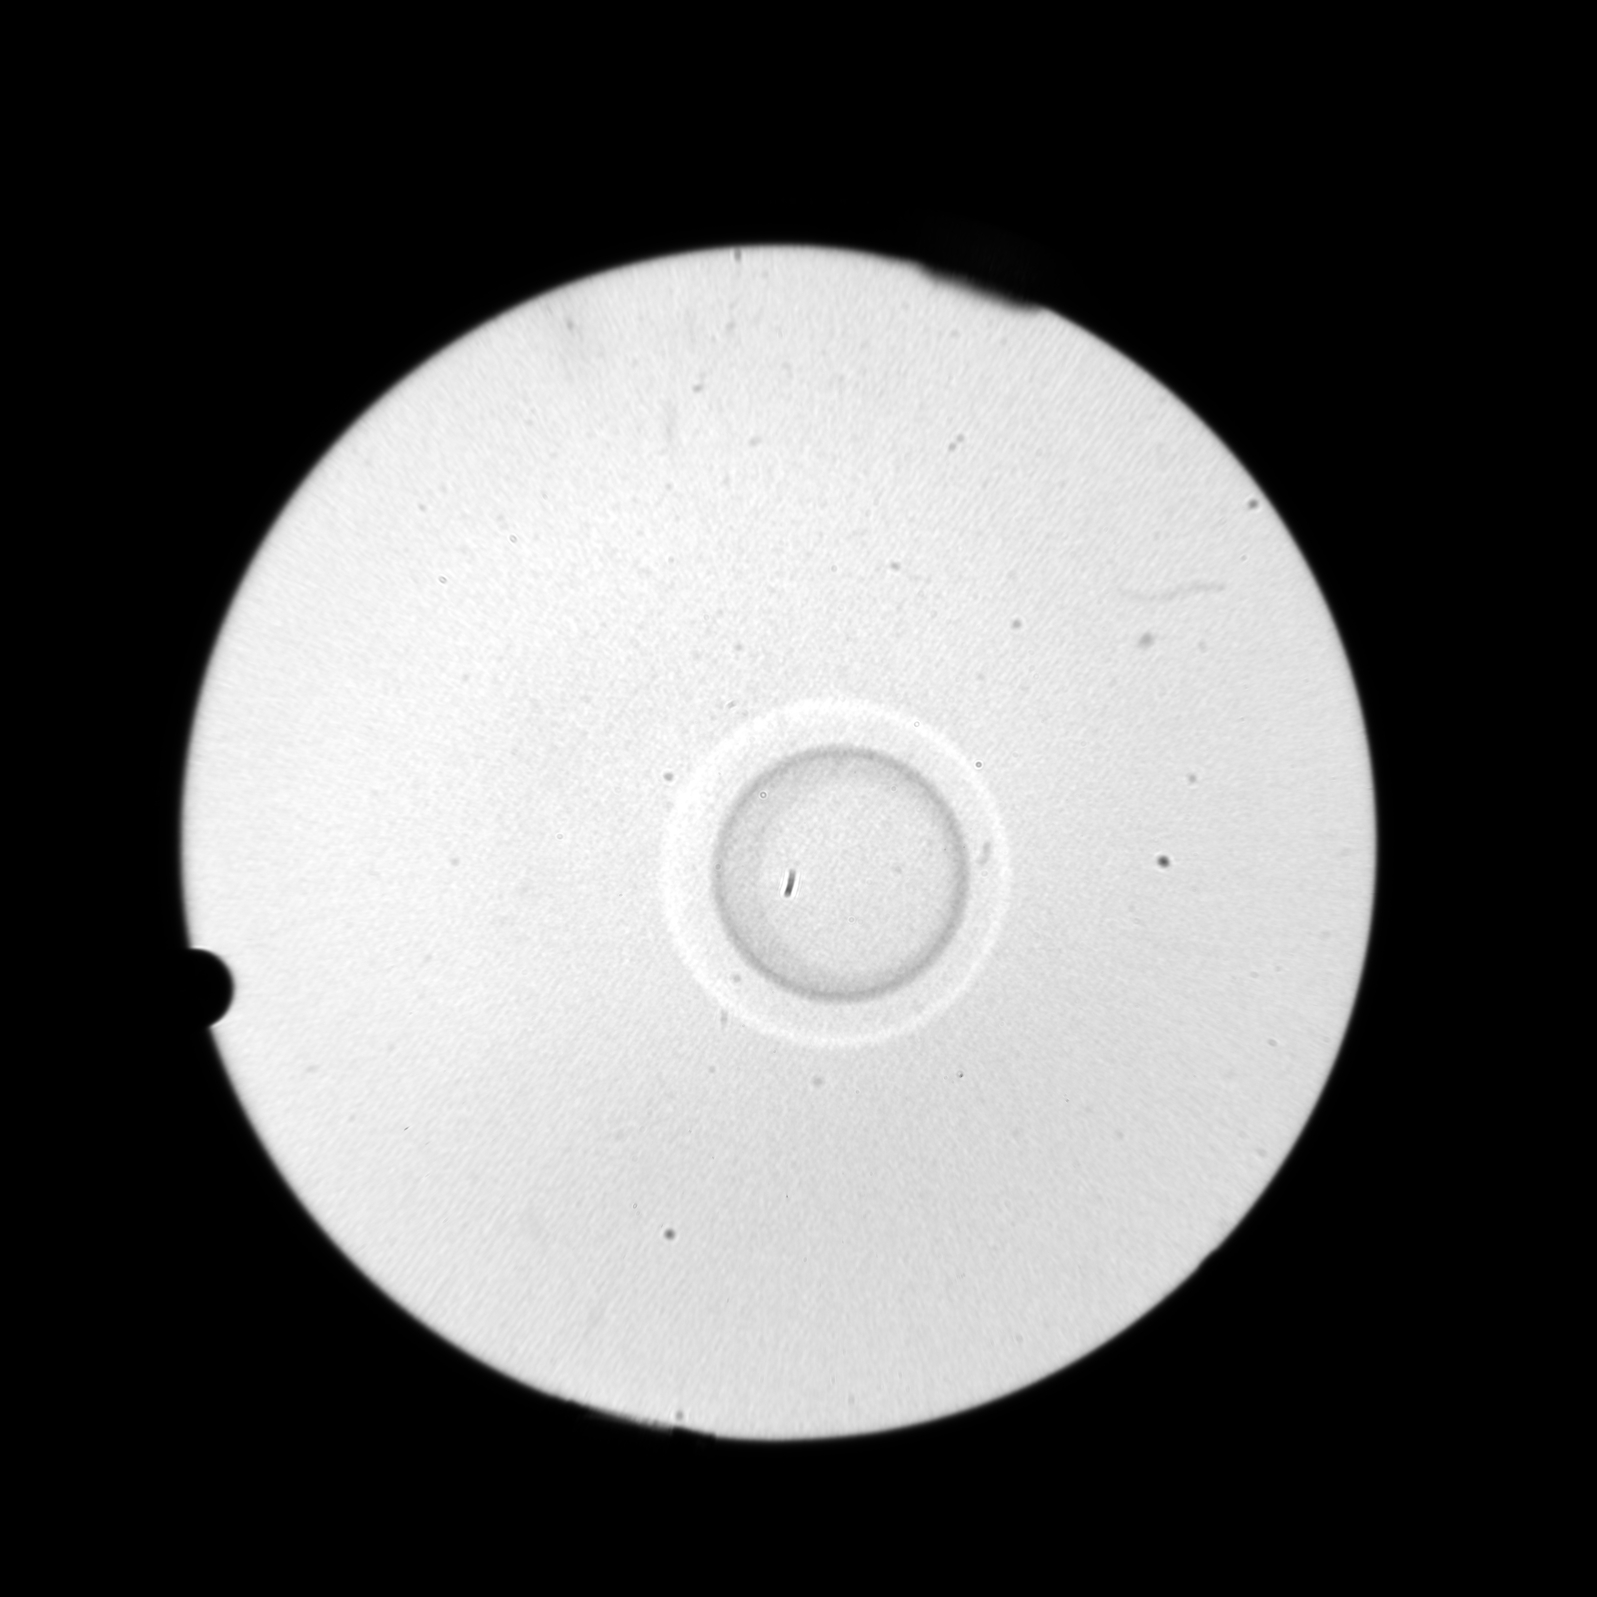
\includegraphics[width=0.5\linewidth]{images/og-wooptix.png}
    \caption{Original Wooptix sample image.}
    \label{fig:og-wooptix}
\end{figure}

The following testing will be performed using a 8 by 8 circle-shaped structuring element, represented in Listing \ref{listing:circle-se}, whose chosen center is (3, 3) or the fourth element of the fourth row.

\begin{tabular}{c}
\lstinputlisting[language=C++,style=cppstyle,caption={Circle-shaped structuring element.},label={listing:circle-se}]{listings/circle.txt}
\end{tabular}

The result of the operation can be observed in Figure \ref{fig:result-wooptix}, distinguishing the original image from the eroded one.
Although it appears to be a minor change, the difference can be seen by observing the dark spot near the center of the image.

\begin{figure}[H]
    \centering
    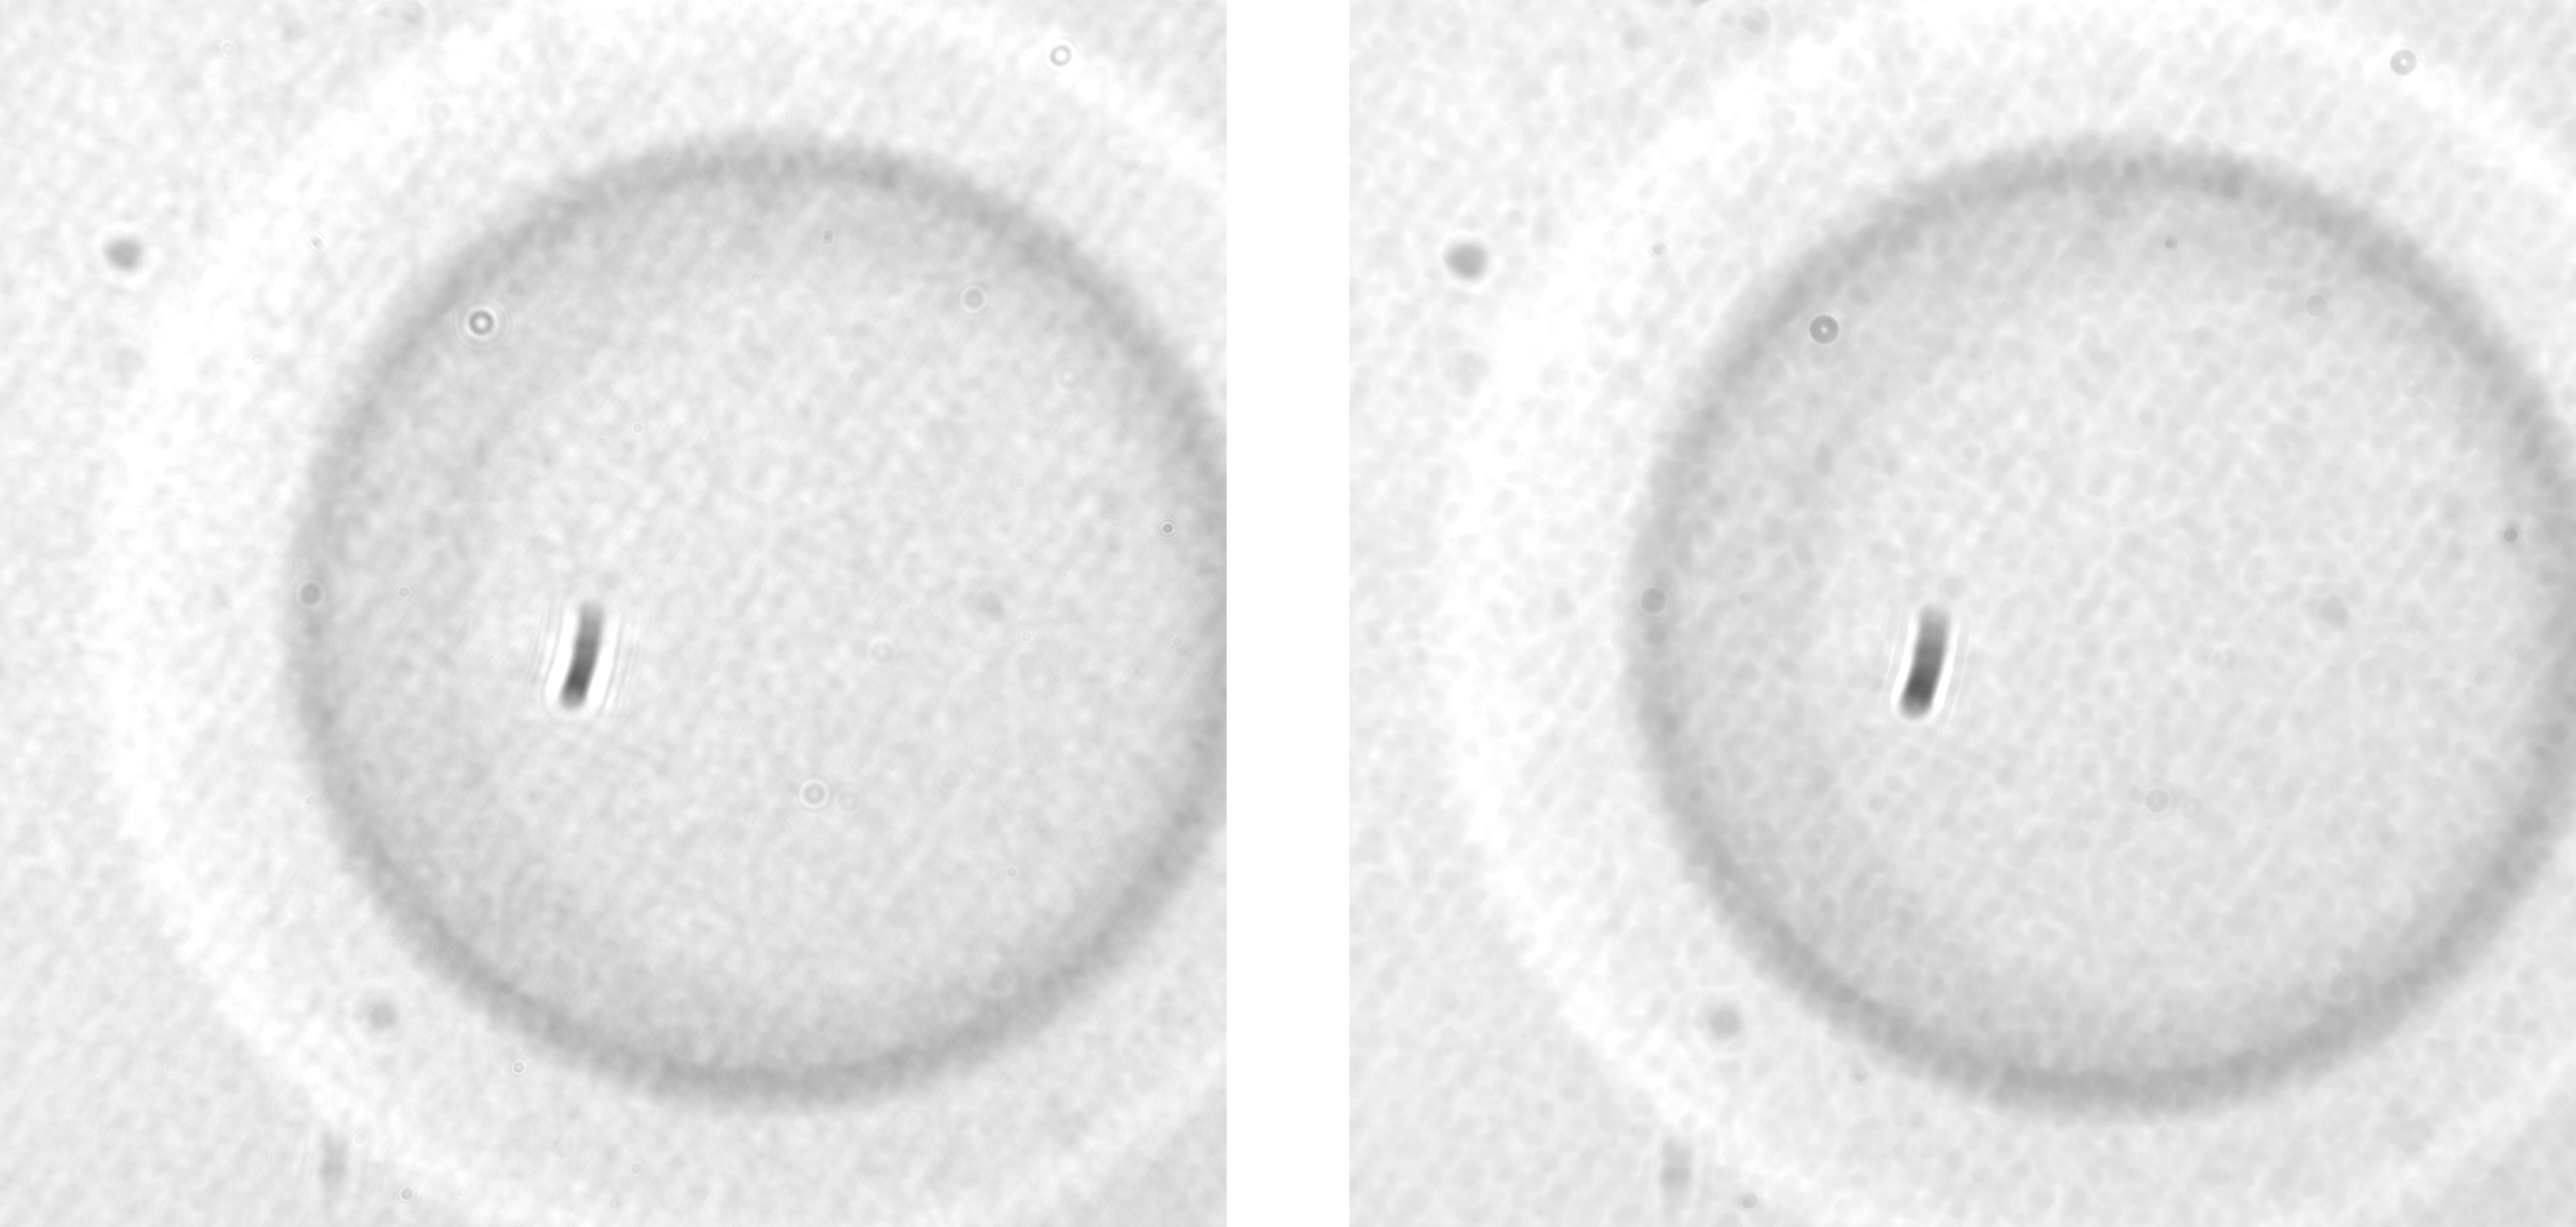
\includegraphics[width=0.7\linewidth]{images/comparison-wooptix.png}
    \caption{Zoomed in Wooptix sample image. Original (left) and eroded (right).}
    \label{fig:result-wooptix}
\end{figure}

Once again, executing the algorithm 10 times and averaging the resulting times, we can see the following differences in time:

\begin{itemize}
    \item The overall program execution time is 58.61 seconds for serial and 56.30 seconds for SYCL.
    \item The operation execution time is 3.32 seconds for serial and 0.29 seconds for SYCL.
\end{itemize}

Considering all 10 execution instances, the overall program execution time varies from 45 to 70 seconds for both serial and SYCL implementations.
On the other hand, the SYCL version clearly outperforms the serial version when it comes to the execution of the erosion operation itself, gaining a speed-up of factor 11.5.
